\documentclass{article}
\usepackage[utf8]{inputenc}
\usepackage[T1]{fontenc}
\usepackage[english]{babel}
\usepackage{amsmath}
\usepackage{amssymb,amsfonts,textcomp}
\usepackage{array}
\usepackage{hhline}
\usepackage{hyperref}
\usepackage{graphicx}     

\let\oldsection\section
\renewcommand\section{\clearpage\oldsection}

\graphicspath{ {./images/} }

\begin{document}
	\title{Croud \\ \vspace{2 mm} {\large A non-technical geographic crowdsourcing framework}}
	\author{Samuel Gaus}
	\date{1st May 2015}
	\maketitle

	\tableofcontents

	\section{Summary}
	\label{sec:summary}
		Geographical data collection is a commonly-repeated task in scientific research, political campaigning, land administration and humanitarian projects.
		At the moment, there are a number of solutions for organisations wishing to go about data collection, from using existing frameworks to commissioning bespoke software.
		However, these are either extremely technical, overly generic (i.e. not specifically suited to collecting geographic point data) or expensive to implement.

		In this document I will show that in essence most organisations have very similar requirements for their data collection and as such it is possible to engineer a solution that is abstract enough to be used in many different fields.
		After analysing a number of potential benefactors, I produced a framework, set of APIs and mobile app that can be used by anyone requiring a crowdsourcing campaign to start collecting data in minutes.

		The framework I have produced could be applied to collecting data on potholes just as easily as it could be used to help volunteers map out crisis-prone areas of the world.

	\section{Introduction}
	\label{sec:introduction}
		\subsection{Problem}
		Data collection is a very common task in computer science and software development. The requirement to gather information from disparate human sources (or crowdsourcing) can be found from everywhere research projects to humanitarian missions.

		\subsection{Status Quo}
		At the moment individuals or organisations looking to initiate a campaign of data collection either have to start their project from scratch or use one of the extremely abstract frameworks available.
		The framework with the widest reach is \textit{PyBOSSA}, a crowdsourcing platform inspired by \textit{BOSSA} and written in Python. \textit{BOSSA} is a frontend written in PHP to provide a web-based client for \textit{BOINC}, the software behind hundreds of data collection projects such as \textit{SETI@home}, \textit{World Community Grid} and \textit{Climate Prediction}\cite{_boinc_2015}.
		PyBOSSA is a rewrite of that with a focus on helping scientists and other researchers crowdsource human problem-solving skills.

		Alternatively, some organisations have produced their own bespoke software. In 2007, \textit{mySociety} made FixMyStreet - a platform for ``reporting common street problems such as potholes and broken street lights''\cite{_mysociety/fixmystreet_2015}.
		A user needs only to click on a map, fill in a survey and submit and the report is sent to the relevant council authority.
		This system was released open-source for any council to host and use, and theoretically for anyone to adapt to their own crowdsourcing needs.

		There are a number of issues present in using the existing solutions of \textit{PyBOSSA}, \textit{FixMyStreet} or bespoke software. Firstly, for all three there is a technical knowledge requirement. \textit{PyBOSSA} and \textit{FixMyStreet} both need server space, system administration to install and maintain and all the skills required for any necessary customisations.
		\textit{crowdcrafting} is a platform powered by the \textit{PyBOSSA} framework which is free to use and allows a user to set up a \textit{PyBOSSA} campaign without the aforementioned requirements.
		However, even in this case, there is significant technical knowledge requried to set up a geographic data-collection campaign due in part to the level of abstraction that the project has achieved from the types of data it could be used to collect.
		A campaign creator must create a form in \textit{HTML} for the data collection, and the user does not get easy access to a map to just drop their pin. Requiring technical skill to operate the software means that in order to run a campaign one either needs a specific skillset or the financial resources necessary to pay a third party.

		There is no way to validate data input using this methid.
		For example, you may have a field of data collection in your campaign that must be numerical.
		Although you can use the \texttt{number} input type in \textit{HTML}, this doesn't stop an old browser or malicious user sending non-numerical data in the response.

		The data submission in \textit{PyBOSSA} is very much a one-way street in terms of availability. By this I mean that the data visibility is low for the user and high for the campaign owners. Many crowdsourcing solutions (for example FixMyStreet) have a much more balanced data visibility, where both users and owners can see the data that has been submitted so far.

		Finally, although existing systems could be used hypothetically with enough technical skill for most crowdsourcing campaigns, they would still take a lot of time to prepare. In some applications of crowdsourced data collection time taken to set up a campaign is an extremely important factor. For example, when Malaysian Airlines Flight 370 crashed in 2014, there was an immediate rush of humanitarian workers to find the location of the plane. Enormous stretches of sea were inspected remotely by ``citizen scientists'' within days due to the existence of \textit{Tomnod} - a crowdsourcing platform built around distributed human inspection of images (in this case satellite images)\cite{_missing_2014}. Because a crowdsourcing framework was already in place specifically for that sort of data analysis, they were able to be more responsive than the government organisations expending huge resource on similar endeavours.

		\subsection{Proposal}
		In the previous sections we have seen that there a number of projects that have been created to crowdsource data from users in the field. We have also seen from \textit{Tomnod} that pre-existing frameworks that are highly specialised are extremely important for easily setting up data collection campaigns quickly and cheaply. Would it be possible to create a framework targeted and tailored specifically for distributed data collection in the field?

		\subsection{Structure}
		In this document I will show that it is indeed possible to create an easy-to-use, quick and open crowdsourcing framework. I will show tha when the data collection requirements are focussed on geographic data, efforts from anyone looking to crowdsource could be reduced dramatically.

		First I will explore the \hyperref[sec:background]{background} of crowdsourcing and ``citizen science'' in more depth. I will assess a number of projects that could benefit from a common framework and determine the common functionalities. I will compare these functionalities with the features of currently-available frameworks and will show, as a result that the framework I propose would be an original work benefiting users and campaign-creators alike.

		Once the set of required features is clear, I will go into more detail about the \hyperref[sec:architecture]{architecture} I use to create such a framework. I will give a more detailed explanation of what the framework actually is and supply a comprehensive requirements analysis to which the project could be built. I will show how the diffrent components fit together and how it works overall. I will then elaborate on and justify the specific technologies I have implemented.

		I will then give more information on the actual \hyperref[sec:implementation]{implementation} of the software complete with source code. I will go through the schemas used in the data storage and some key snippets from the source code. I will also provide information on some of the features that would be more challenging for someone attempting to reproduce the framework themselves.

		In order to show that the framework is appropriately constructed, I will \hyperref[sec:evaluation]{evaluate} it against two completely separate potential campaigns and show that it is suited to the requirements of both. In this section I will walk through the creation of a campaign with screenshots, and then do the same for submitting data to a campaign.

		In \hyperref[sec:conclusion]{conclusion}, I will explore and recommend some future improvements on the framework and associated applications and will provide an analysis on what worked and why.

		The software I produced to show this is called \textit{croud}, a portmanteau of ``cloud'' and ``crowd''. It is hosted on \href{http://croud.io/}{\texttt{http://croud.io/}} - please feel free to visit and try it out for yourself.

	\section{Background}
	\label{sec:background}
		\subsection{Crowdsourcing}
		Crowdsourcing is a term coined in 2005 by editors of \textit{Wired Magazine} Jeff Howe and Mark Robinson\cite{safire_fat_2009} referring to the outsourcing of a task to the crowd. The rise of the internet and of mobile phones has made crowdsourcing an extremely efficient way of collecting data on a large scale. Due in part to its relevance to both business and academic research, it has been subject to a vast quantity of study of both its effectiveness\cite{brabham_effectiveness_2010} and the techniques of motivation that draw people to participating\cite{hossain_users_2012}. Much of this study is part of research focussing on \textit{computer-supported cooperative work}, a more general topic covering software that helps groups of people work together in ways that would not be possible or worthwhile without technology.

		When applied to gathering data for research, crowdsourcing is a form of citizen science\cite{_citizen_2015}. In this field, however, there is a more specific definition given to crowdsourcing. Muki Halay describes crowdsourcing as ``level 1'' of participation in citizen science, where a citizen merely acts a sensor. In higher levels, citizens contribute to data interpretation (``distributed intelligence''), problem definition (``participatory science'') and data analysis (``extreme citizen science'')\cite{haklay_citizen_2013}.

		\subsection{Existing projects}
		There are a growing number of projects that involve crowdsourcing geographic information. Although there are many to choose from, I will provide information for a few that I believe represent the disparate use cases.

		\paragraph{OpenStreetMap}
		\textit{OpenStreetMap} (\textit{OSM}) is a world-wide online collaborative effort to create detailed maps of the world under a free\cite{_open_2012} license started in 2004. Any user from around the world can submit geographic data using either the web-based application, or offline tools like \textit{Merkaartor}. Although used by individuals and organisations everywhere, it has also been crucial in ``crisis mapping''. Since the Haiti earthquate in 2010, volunteers have provided geographic data on areas experiencing crises to \textit{OSM} to help humanitarian workers\cite{_our_????}. This effort has since expanded into the Missing Maps project, within which the \textit{Humanitarian OSM Team} work with \textit{Medecins Sans Frontieres} and the \textit{American Red Cross} to preemptively map ``the most crisis-prone parts of the developing world''\cite{_missing_????}.

		\paragraph{FixMyStreet}
		\textit{FixMyStreet} is - a platform for ``reporting common street problems such as potholes and broken street lights''\cite{_mysociety/fixmystreet_2015} created by \textit{mySociety} in 2007. \textit{mySociety} is an ``e-democracy'' charity in the UK that have created and operate a number of tools to improve the user experience of national and local government. \textit{FixMyStreet} in particular is used to simplify the process of reporting potholes, broken streetlamps etc. to their local authority. Users submit a description of the problem attached to a coordinate pair via the website or apps for \textit{Android} and \textit{iOS}. It has been adopted by local authorities all over the world.

		\paragraph{Fill That Hole}
		\textit{Fill That Hole} is a cyclist-specific app for reporting potholes to the relevant Council in the UK. It differs from other reporting systems because the data submitted is public and freely usable by other systems via and API. For example, the journey planner \textit{Cyclestreets} takes the potholes reported on \textit{Fill That Hole} into account when planning routes. Reports are submitted via apps for \textit{Android} and \textit{iOS}.

		\paragraph{Cyclestreets}
		Although basing most of its data on \textit{OSM}, the cyclist journey planner \textit{Cyclestreets} also hosts a photomap where users are encourage to upload geolocated photographs of cycling infrastructure to their ``Photomap''. This data is used to affect route planning and the prooided images themselves are appended to route itineraries\cite{_cyclestreets_????}.

		\subsubsection{Common functionalities}

		The projects listed above share a number of functionalities. I have isolated and listed them here, although every project does not require every functionality.

		\begin{itemize}
			\item Interface to submit some validated payload of data with an accompanying coordinate pair.
			\item Some means of displaying the submitted data on a map. This may be as a set of markers, icons or a heatmap.
			\item Ability to export the collected data in a machine-readable format.
			\item When data is submitted by anonymous or unknown users, it may require moderation either due to being false, because it needs editing or because the data is no longer relevant.
			\item A well documented API covering all of this functionality. Typically these tools exist as part of a chain of software; they need a good machine interface to be able to receive data in as many ways as possible, and to share their collected data as required.
		\end{itemize}

		\subsection{Available frameworks}

		The field of crowdsourcing is not without existing frameworks. The key offering currently available is \textit{PyBOSSA}, already introduced in section \ref{sec:introduction}. However, the framework is not compatable with the field of crowdsourcing projects addressed in this study. This will be made clear in the walkthrough below.

		\subsubsection{Walkthrough}

		\textit{PyBOSSA} is available without requiring server space through \textit{crowdcrafting}. I will cover briefly the process for creating a geographic in-the-field data collection project using \textit{crowdcrafting}.

		\begin{enumerate}
			\item Create a user account on the webiste.
			\item Start a new `Project' (see Figure \ref{fig:cc-create}).
			\item `Import' some `Tasks'.\\
			\textit{crowdcrafting} is designed to atomize tasks and distribute them between contributors. In order to achieve this, it requires a CSV (or Google Spreadsheet or similar) of `Tasks'. For example, in the geographic data example they provide for ``Urban Parks'', the tasks are questions like ``Find an urban park for this city'', along with a city name\cite{_urban_????}. To make the system cater for the kind of campaign discussed in this project, the file provided here would need to be consist of a singular question.
			\item Edit the `Task Presenter' to be both mobile-compatable and capable of using geolocation as well as pointing to where you are on a map.
			\item Publish the Project.
		\end{enumerate}

		\begin{figure}[hb]
			\centering
			\fbox{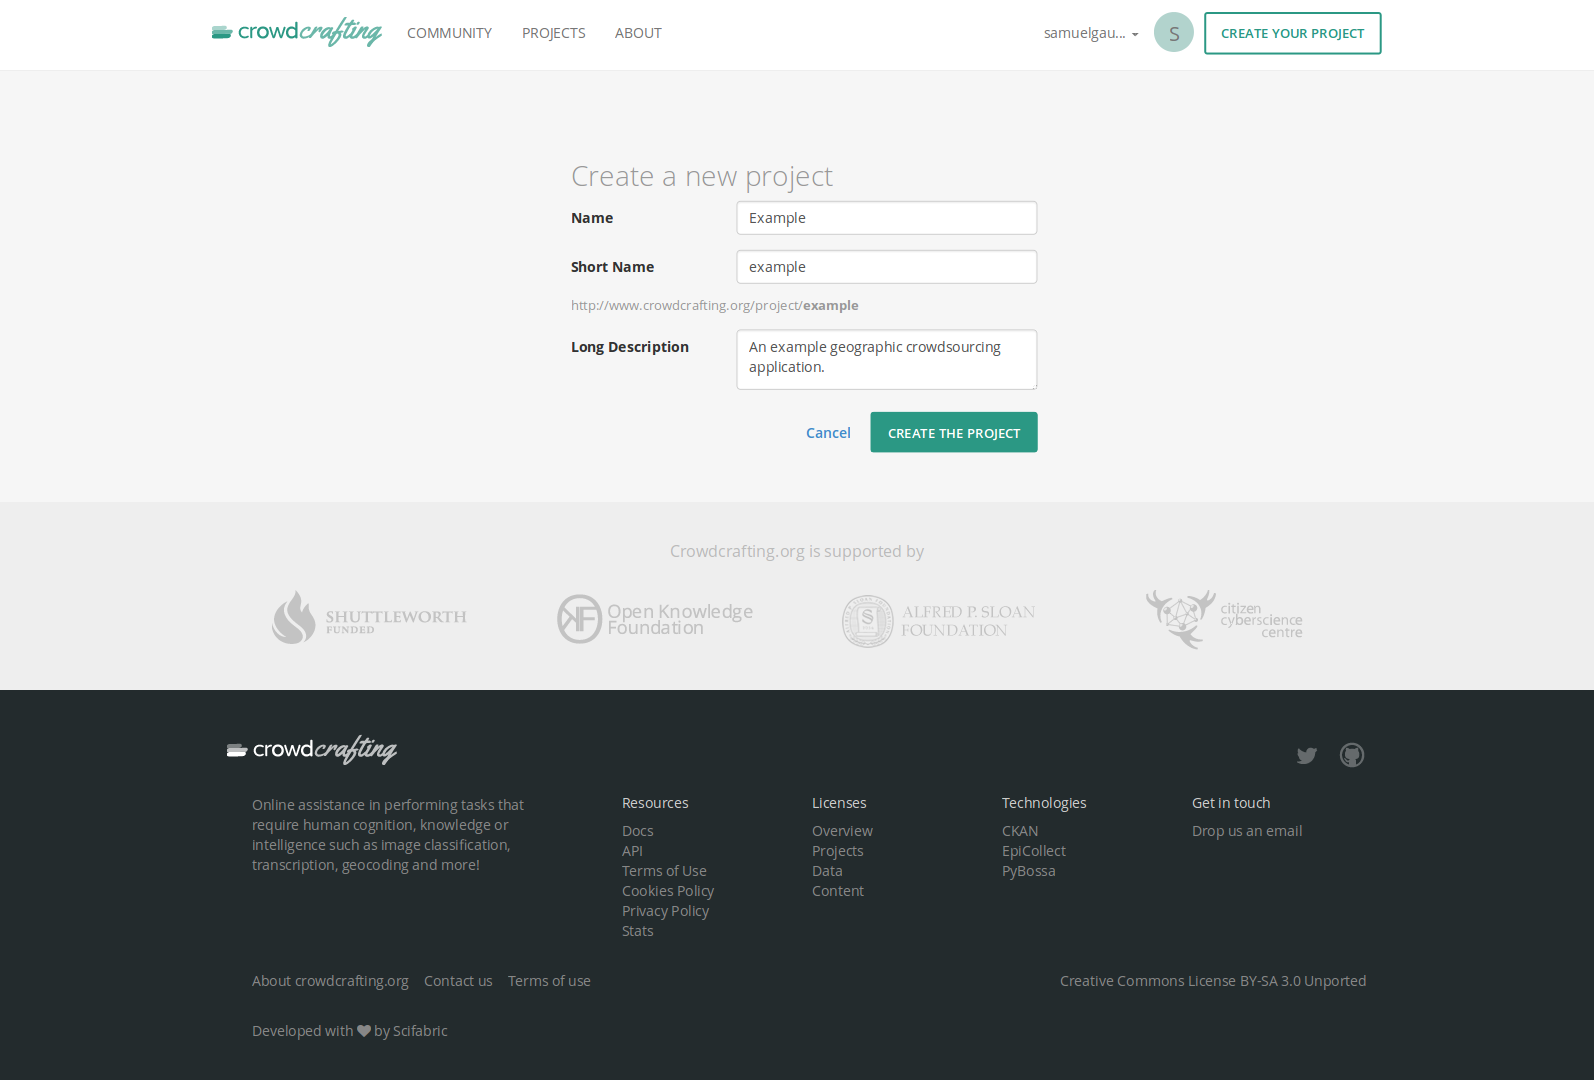
\includegraphics[width=4in]{cc-create}}
			\caption{Creating a project in \textit{crowdcrafting}}
			\label{fig:cc-create}
		\end{figure}

		This would then create an input form for the data you wish to collect. However, because \textit{PyBOSSA} focusses on atomised tasks rather than a more general goal, it is not possible to create a question that any user can repeatably answer. For example if you wanted to collect information about potholes, the task ``Where do you see a pothole?'' could be created. Once a user has `completed' this `task', however, they would not be able to answer it again, this causing the campaign to almost be one-use. Similarly, in the `Task Redundancy' settings area, you can specify how many times a single task can be repeated before closing. In the campaigns \textit{PyBOSSA} is built for, this would be to allow verification of submissions by seeing that mmultiple users provided the same data. In our example, however, it would be necessary to provide an arbitrary high number to allow the data collection to continue indefinitely.

		\begin{itemize}
			\item What is available
			\begin{itemize}
				\item PyBossa and free implementation
				\item There is another but I cant remember it and it's shit.
			\end{itemize}
			\item Level of abstraction for non IT people is required. Potentially alleviates need for money and time.
		\end{itemize}

	\section{Architecture}
	\label{sec:architecture}
		\begin{itemize}
			\item What the project is
			\item Requirements analysis - very fine detail. Almost like an API per requirement. Basically walk through actions and almost describe each API call that would need to happen (kind of).
			\item Component diagram. Do not specify technologies (this is for later).
			\item How it works.
			\item Technologies used and why.
			\item Describe Full API docs in appendices.
		\end{itemize}

	\section{Implementation}
	\label{sec:implementation}
		\begin{itemize}
			\item Link to repository.
			\item Link to a working implementation. http://croud.io/.
			\item JSON schema.
			\item Key snippets of code for each component - for each component show a frontend screen and maybe some code that powers it.
			\item Special features that might take effort from new developers.
			\begin{itemize}
				\item Offline caching
				\item Moderation
				\item Stale.
			\end{itemize}
		\end{itemize}

	\section{Evaluation}
	\label{sec:evaluation}
		\begin{itemize}
			\item Show it using two completely different campaigns.
			\item Explain why you chose the two campaigns you did and list their requirements.
			\item Walkthrough of how user would create a campaign (with screenshots and links ideally)
			\item Walkthrough of how data is submitted
		\end{itemize}
	\section{Conclusion}
	\label{sec:conclusion}
		\begin{itemize}
			\item Future changes that could be added.
			\item Conclude that it works etc etc
		\end{itemize}

	\bibliographystyle{Croud}
	\bibliography{Croud}

\end{document}
